\documentclass{beamer}
\usepackage[utf8]{inputenc}
\usetheme{Copenhagen}
\usecolortheme{beaver}
\usepackage{graphicx}

%\setbeamersize{text margin left=2pt,text margin right=2pt} 
\newcommand\Wider[2][3em]{%
	\makebox[\linewidth][c]{%
		\begin{minipage}{\dimexpr\textwidth+#1\relax}
			\raggedright#2
		\end{minipage}%
	}%
}

\newcommand\Wide[2][1.5em]{%
	\makebox[\linewidth][c]{%
		\begin{minipage}{\dimexpr\textwidth+#1\relax}
			\raggedright#2
		\end{minipage}%
	}%
}

\makeatletter
\setbeamertemplate{footline}
{
	\leavevmode%
	\hbox{%
		\begin{beamercolorbox}[wd=0.75\paperwidth,ht=2.25ex,dp=1ex,left]{title in head/foot}%
			\usebeamerfont{title in head/foot}\insertshorttitle{}
		\end{beamercolorbox}%
		\begin{beamercolorbox}[wd=0.25\paperwidth,ht=2.25ex,dp=1ex,right]{date in head/foot}%
			\insertframenumber{} / \inserttotalframenumber\hspace*{2ex} 
		\end{beamercolorbox}}%
		\vskip0pt%
}
\makeatother
 
 
%Information to be included in the title page:
\title[A Comparison of Posterior Approximation Algorithms for LDA]{A Comparison of Posterior Approximation Algorithms for Latent Dirichlet Allocation}
\author{Cindy Cook}
\institute{STAT540:  Final Project}
\date{9 December 2015}
 

\begin{document}
 
\frame{\titlepage}
 
\begin{frame}
\frametitle{Latent Dirichlet Allocation}
\Wider{
\large{Given a corpus $C$, what we know,} \\ \centering{\small{the vocabulary, $V=\{w_{d,n}\}$ and the number of topics $K.$}}
\vspace{5mm}
\begin{columns}
	
	\column{0.6\textwidth}
	\begin{figure}[ht!]
		\centering
		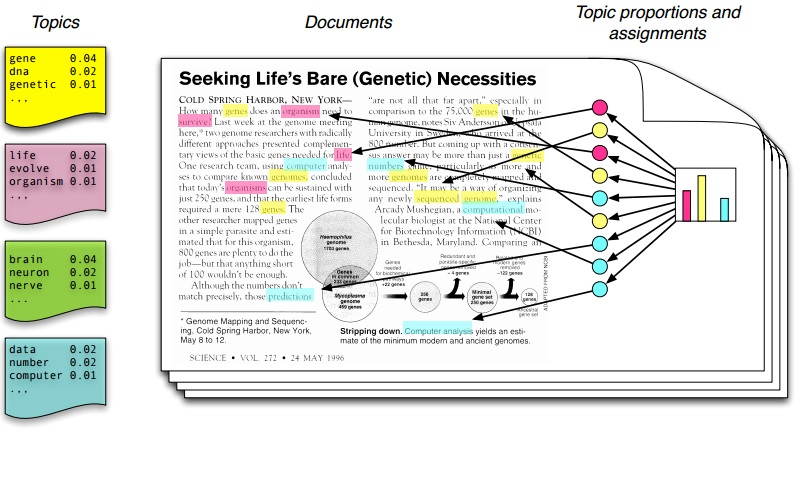
\includegraphics[width=70mm,height=55mm]{LDA.jpg}
		\vspace{-5mm}
		\caption{\tiny{Article from the \textit{Journal of Science}; Image from David Blei's 2012 topic model video lecture series.}}
	\end{figure}
	
	\column{0.4\textwidth}
	\begin{itemize}
		\item Each \textbf{topic} $k$ is a distribution over the vocabulary.
		\item Each \textbf{document} $d$ is a mixture of corpus wide topics.
		\item Each \textbf{word} $w_{d,n}$ is drawn from one of these topics.
	\end{itemize}
\end{columns}
}
\end{frame}


\begin{frame}
	\frametitle{Latent Dirichlet Allocation}
\Wide{
	\begin{columns}
		\column{0.45\textwidth}
		\begin{alertblock}{Generative Process:}
			\begin{itemize}
				\item For each topic $k$: \\
				$\beta^{k} \sim Dir(\eta)$ 
				\item For each document $d$:
				\begin{itemize}
					\item $\theta^{d} \sim Dir(\alpha)$
					\item For each $w_{d,n}$ in $d$:
					\begin{itemize}
						\item Draw $z_{d,n} \sim Multi(\theta^{d})$
						\item Draw $w_{d,n} \sim Multi(\beta^{z_{d,n}})$
					\end{itemize}
				\end{itemize}
			\end{itemize}
		\end{alertblock}
		\column{0.55\textwidth}
		\begin{block}{Prior:}
			$p(\beta, \theta | \eta, \alpha)=p(\beta | \eta)p(\theta | \alpha)$
		\end{block}
		\begin{block}{Likelihood:}
			$p(w | \beta, \theta)=\sum_{z}{(p(w | z, \beta))p(z | \theta)}$
		\end{block}
		\begin{block}{Posterior:}
			$p(\beta, \theta | w, \eta, \alpha)=\frac{p(\beta, \theta | \eta, \alpha)p(w | \beta, \theta)}{ \int_{\beta}\int_{\theta}{ \left[ (p(\beta | \eta)p(\theta | \alpha) \sum_{z}{(p(w | z, \beta)p(z |\theta) ) } ) \right] d\beta d\theta} }$
		\end{block}
	\end{columns}
	\begin{figure}[ht!]
		\centering
		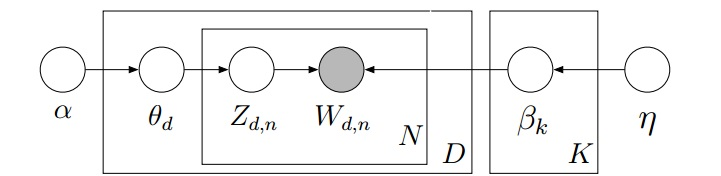
\includegraphics[width=70mm]{LDA2.jpg}
		\vspace{-3mm}
		\caption{\tiny{Directed Graphical Model}}
	\end{figure}
}
\end{frame}


\begin{frame}
	\frametitle{Variational EM}
\Wide{
	\begin{columns}
	\column{0.55\textwidth}
	\small{In general since the posterior $p(\phi | Y)$  is intractable we use a surrogate $q(\phi).$  
		\begin{enumerate}
			\item From Jensen's inequality \textcolor{red}{$\log{p(Y)}\geq\int{(q(\phi)\log{( \frac{p(\phi,Y)} {q(\phi)} )} d\phi ) }=L(q).$} 
			\item From (Bishop, 2006) \textcolor{red}{$\log{p(Y)}=L(q)+KL(q || p).$}  
			\item Finding $q(\phi)$
			\begin{enumerate}
				\item Exponential family assumptions:
				\vspace{-3mm}
				\begin{enumerate}
					\item $p(\phi_{k} | Y, \phi_{-k}) \sim$ exp. family 
					\item $q(\phi_{k}) \sim$ same exp. family
				\end{enumerate}
				\item Mean field assumption:
				\textcolor{blue}{$q(\phi)=\prod_{k=1}^{K}{q(\phi_{k})}.$}
			\end{enumerate}
			\item After some calculus, parameters which minimize KL dist can be iteratively found: \\ \textcolor{blue}{$q(\phi_{k}^{new}) = \frac{ \exp{( E_{j\neq k} [ \log{p(\phi,Y)} ] )} }{ \int{ \exp{( E_{j\neq k} [ \log{p(\phi,Y)} ] )} d\phi_{k} } }$.} 
		\end{enumerate}
	}	
	\column{0.45\textwidth}
	\small{
	$q(\phi)=\prod_{k=1}^{K}{q(\beta | \tilde{\eta})}\prod_{d=1}^{D}{q(\theta | \tilde{\alpha})}$ \\ \hspace{12mm}$\prod_{n=1}^{V}{q(z_{d,n} | \tilde{\gamma})}.$
	\begin{block}{Algorithm:}
		\begin{enumerate}
			\item Initialize $\tilde{\eta}^{(0)}, \tilde{\alpha}^{(0)}, \tilde{\gamma}^{(0)}$ 
			\item (E-step) \tiny{Minimize $KL(q || p)$}
			\\ \small{Use coordinate ascent algorithm to optimize parameters.}
			\item (M-step) \tiny{Maximize $L(q)$ wrt $\alpha, \eta, \gamma$}
			\\ \small{Find MLE for $\beta$ from expected counts (i.e. sufficient stats)}
			\item If $L(q)$ converged then stop
			\item Else return to (E-step)
		\end{enumerate}
	\end{block}
	}
	\end{columns}
}
\end{frame}


\begin{frame}
	\frametitle{Collapsed Gibbs Sampling}
\Wide{
	\begin{columns}
		\column{0.55\textwidth}
		\begin{block}{Simple Gibbs Sampler}
			\begin{itemize}
				\item Initialize $\beta^{(0)}, \theta^{(0)}, z^{(0)}_{d,n}$
				\item Repeat until convergence for $t=1,2,...$
					\begin{itemize}
						\item Draw $\beta^{(t+1)} \sim p(\beta^{(t+1)} | z^{(t)}_{d,n}, w_{d,n})$  
						\item Draw $\theta^{(t+1)} \sim p(\theta^{(t+1)} | z^{(t)}_{d,n}, w_{d,n})$
						\item Draw \vspace{-2mm} 
						\begin{align*} 
						z^{(t+1)}_{d,i} \sim p(z^{(t+1)}_{d,i} &| \beta^{(t+1)}, \theta_{d}^{(t+1)}, \\ & z^{(t+1)}_{d,-i}, w_{d,n}) 
						\end{align*}
					\end{itemize} 
			\end{itemize}
		\end{block}
		\small{Simple due to the conjugacy of the priors, but VERY slow!!}
		\column{0.45\textwidth}
		\small{Integrate out $\beta$ and $\theta$.}
		\begin{block}{Collapsed Gibbs Sampler}
			\begin{itemize}
				\item Initialize $z^{(0)}_{d,n}$
				\item Repeat for $t=1,2,...$ 
					\begin{itemize}
						\item Draw $z^{(t+1)}_{d,i} \sim p(z^{(t+1)}_{d,i} | z^{(t+1)}_{d,-i}, w_{d,n})$
					\end{itemize}
				\item Stop when $H(P,Q)<tol$
				\item Solve for $\hat{\beta}$
				\item Solve for $\hat{\theta}$ 
			\end{itemize}
		\end{block}
		\small{Faster, but still slow with large vocabularies.} \\ \small{Asymptomatically accurate.}
	\end{columns}
}
\end{frame}


\begin{frame}
	\frametitle{Simulation Study}
\Wider{
	\small{	
	\vspace{-5mm}
	\begin{itemize}
		\item Simulated 36 $C$'s according to the LDA generative process with:
		\item $D=10$; $\alpha=\eta=\{0.01, 0.1, 1, 10\}$; $K=\{2, 5, 10\}$; $|V|=\{50, 100, 500\}$
	\end{itemize}
	}
\vspace{-10mm}
\begin{columns}
	\column{0.5\textwidth}
	\begin{figure}[ht!]
		\centering
		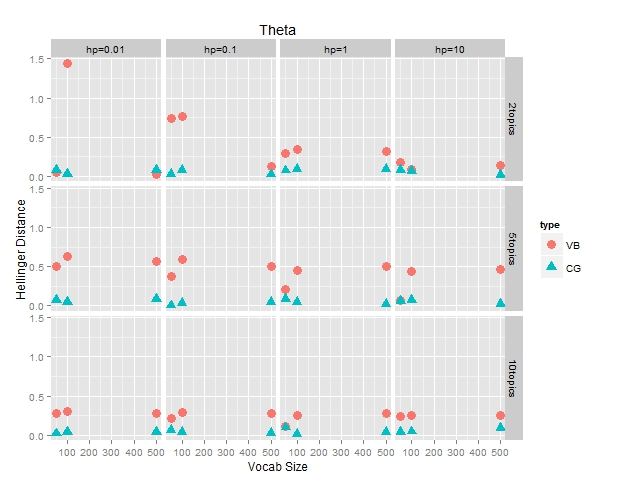
\includegraphics[width=70mm,height=60mm]{Hdist_theta.jpeg}
	\end{figure}
	
	\column{0.5\textwidth}
	\begin{figure}[ht!]
	\centering
	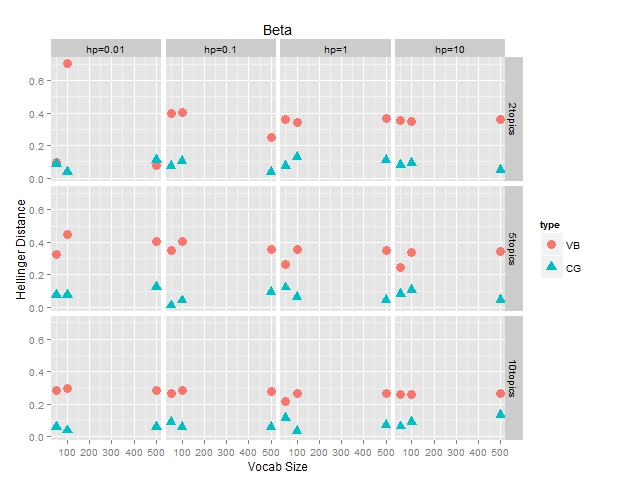
\includegraphics[width=70mm,height=60mm]{Hdist_beta.jpeg}
\end{figure}
\end{columns}
%\tiny{VEM appears to perform better with smaller number of topics, but not consistently across hyper-parameters or vocab size. \\
%	CG consistently gains in performance across hyper-parameter values and vocab size as the number of topics increases.}
}
\end{frame}


\begin{frame}
	\frametitle{Conclusions}
	\begin{itemize}
		\item Discussion: 
		\begin{itemize}
			\item CGS took significantly longer to run then VEM
			\item Need to run CGS longer for smaller values of $K$
			\item VEM is biased for both $\theta$ and $\beta$
			\item Recommend cautiously using VEM if user needs results immediately. If time permits, always use CGS.
		\end{itemize}
		\vspace{5mm}
		\item Future Directions:
		\begin{itemize}
			\item Not a fair comparison; should look into collapsed VEM
			\item Initial Values
			\item LDA may not be appropriate to begin with
		\end{itemize}
	\end{itemize}
\end{frame}
\end{document}